\documentclass[12pt]{article}

\usepackage{caption} %interesting things with captions
\usepackage[margin=1.5in]{geometry} %mostly set margin of the report
\usepackage{tabulary} %text wrapping in tables
\usepackage{subcaption} %let me put multiple images into a single caption
\usepackage{textcomp} %let me use \textrangle{} to get '>'
\usepackage{hyperref} %links in ToC - should be mostly the last thing imported?

%images being embeded
\usepackage{graphicx}
\graphicspath{ {images/} }

%code highlighting
\usepackage{minted}
\setminted[c++]{frame=single,linenos=true,autogobble=true,numbersep=4pt,tabsize=4}
\setminted[bash]{frame=single,linenos=true,autogobble=true,numbersep=4pt,tabsize=4}
\setminted[xml]{frame=single,linenos=true,autogobble=true,numbersep=4pt,tabsize=4}

%fix a quote mark issue
\usepackage [english]{babel}
\usepackage [autostyle, english = american]{csquotes}
\MakeOuterQuote{"}

%page 129
\begin{document}
\pagenumbering{gobble}
\begin{titlepage}
	\centering
	{\Huge Iteration 1\par}
	\vspace{0.25in}
	{\Large Reddit Robot\par}
	\vspace{2in}
	{Alex Harper\par}
	\newpage
\end{titlepage}
\pagenumbering{roman}
\tableofcontents
\newpage
\pagenumbering{arabic}

\section{Use Cases}

This is elaborating on the basic use cases presented in the inception period.

\hypertarget{Authenticate the User}{
\subsection{Authenticate the User}
}
\begin{itemize}
	\item No Refresh Token
	\begin{itemize}
		\item Prompt the user to visit the correct URL (includes scopes and program ID)
		\item Prompt the user to click "Allow" on the webpage
		\item Prompt the user to copy the URL they got redirected to back into the program
		\item Parse the URL for the temperary token
		\item Use the one-time-use token to get the session and refresh tokens
		\item Save the refresh token to disk
		\item Restart the session timeout timer
	\end{itemize}

	\item Has Refresh Token but not Session Token
	\begin{itemize}
		\item Use the refresh token to get a new session token
		\item Restart the session timeout timer
	\end{itemize}

	\item Has Session Token and Refresh Token
	\begin{itemize}
		\item If session timeout timer is past 3600 seconds, use \textit{Has Refresh Token but not Session Token}
	\end{itemize}
\end{itemize}

\subsection{Read Data}
\begin{itemize}
	\item \hyperlink{Authenticate the User}{\textit{Authenticate the User}}
	\item Check that not too many requests have been made in the last time period
	\item Set the HTTP header
	\begin{itemize}
		\item Set the useragent string in the header
		\item Set the authorization string in the header
	\end{itemize}
	\item Make request
	\item Wait for reply to finish
	\item Get information from reply
	\begin{itemize}
		\item Get the \textit{X-Ratelimit-Remaining} number from the header (requests available left)
		\item Get the \textit{X-Ratelimit-Reset} number from the header (time until get more requests)
	\end{itemize}
	\item Return the body of the message

\end{itemize}

\newpage
\section{Domain Diagram}
\begin{figure}[ht]
	\centering
	\caption{The Reddit Domain Diagram}
	\label{domain}
	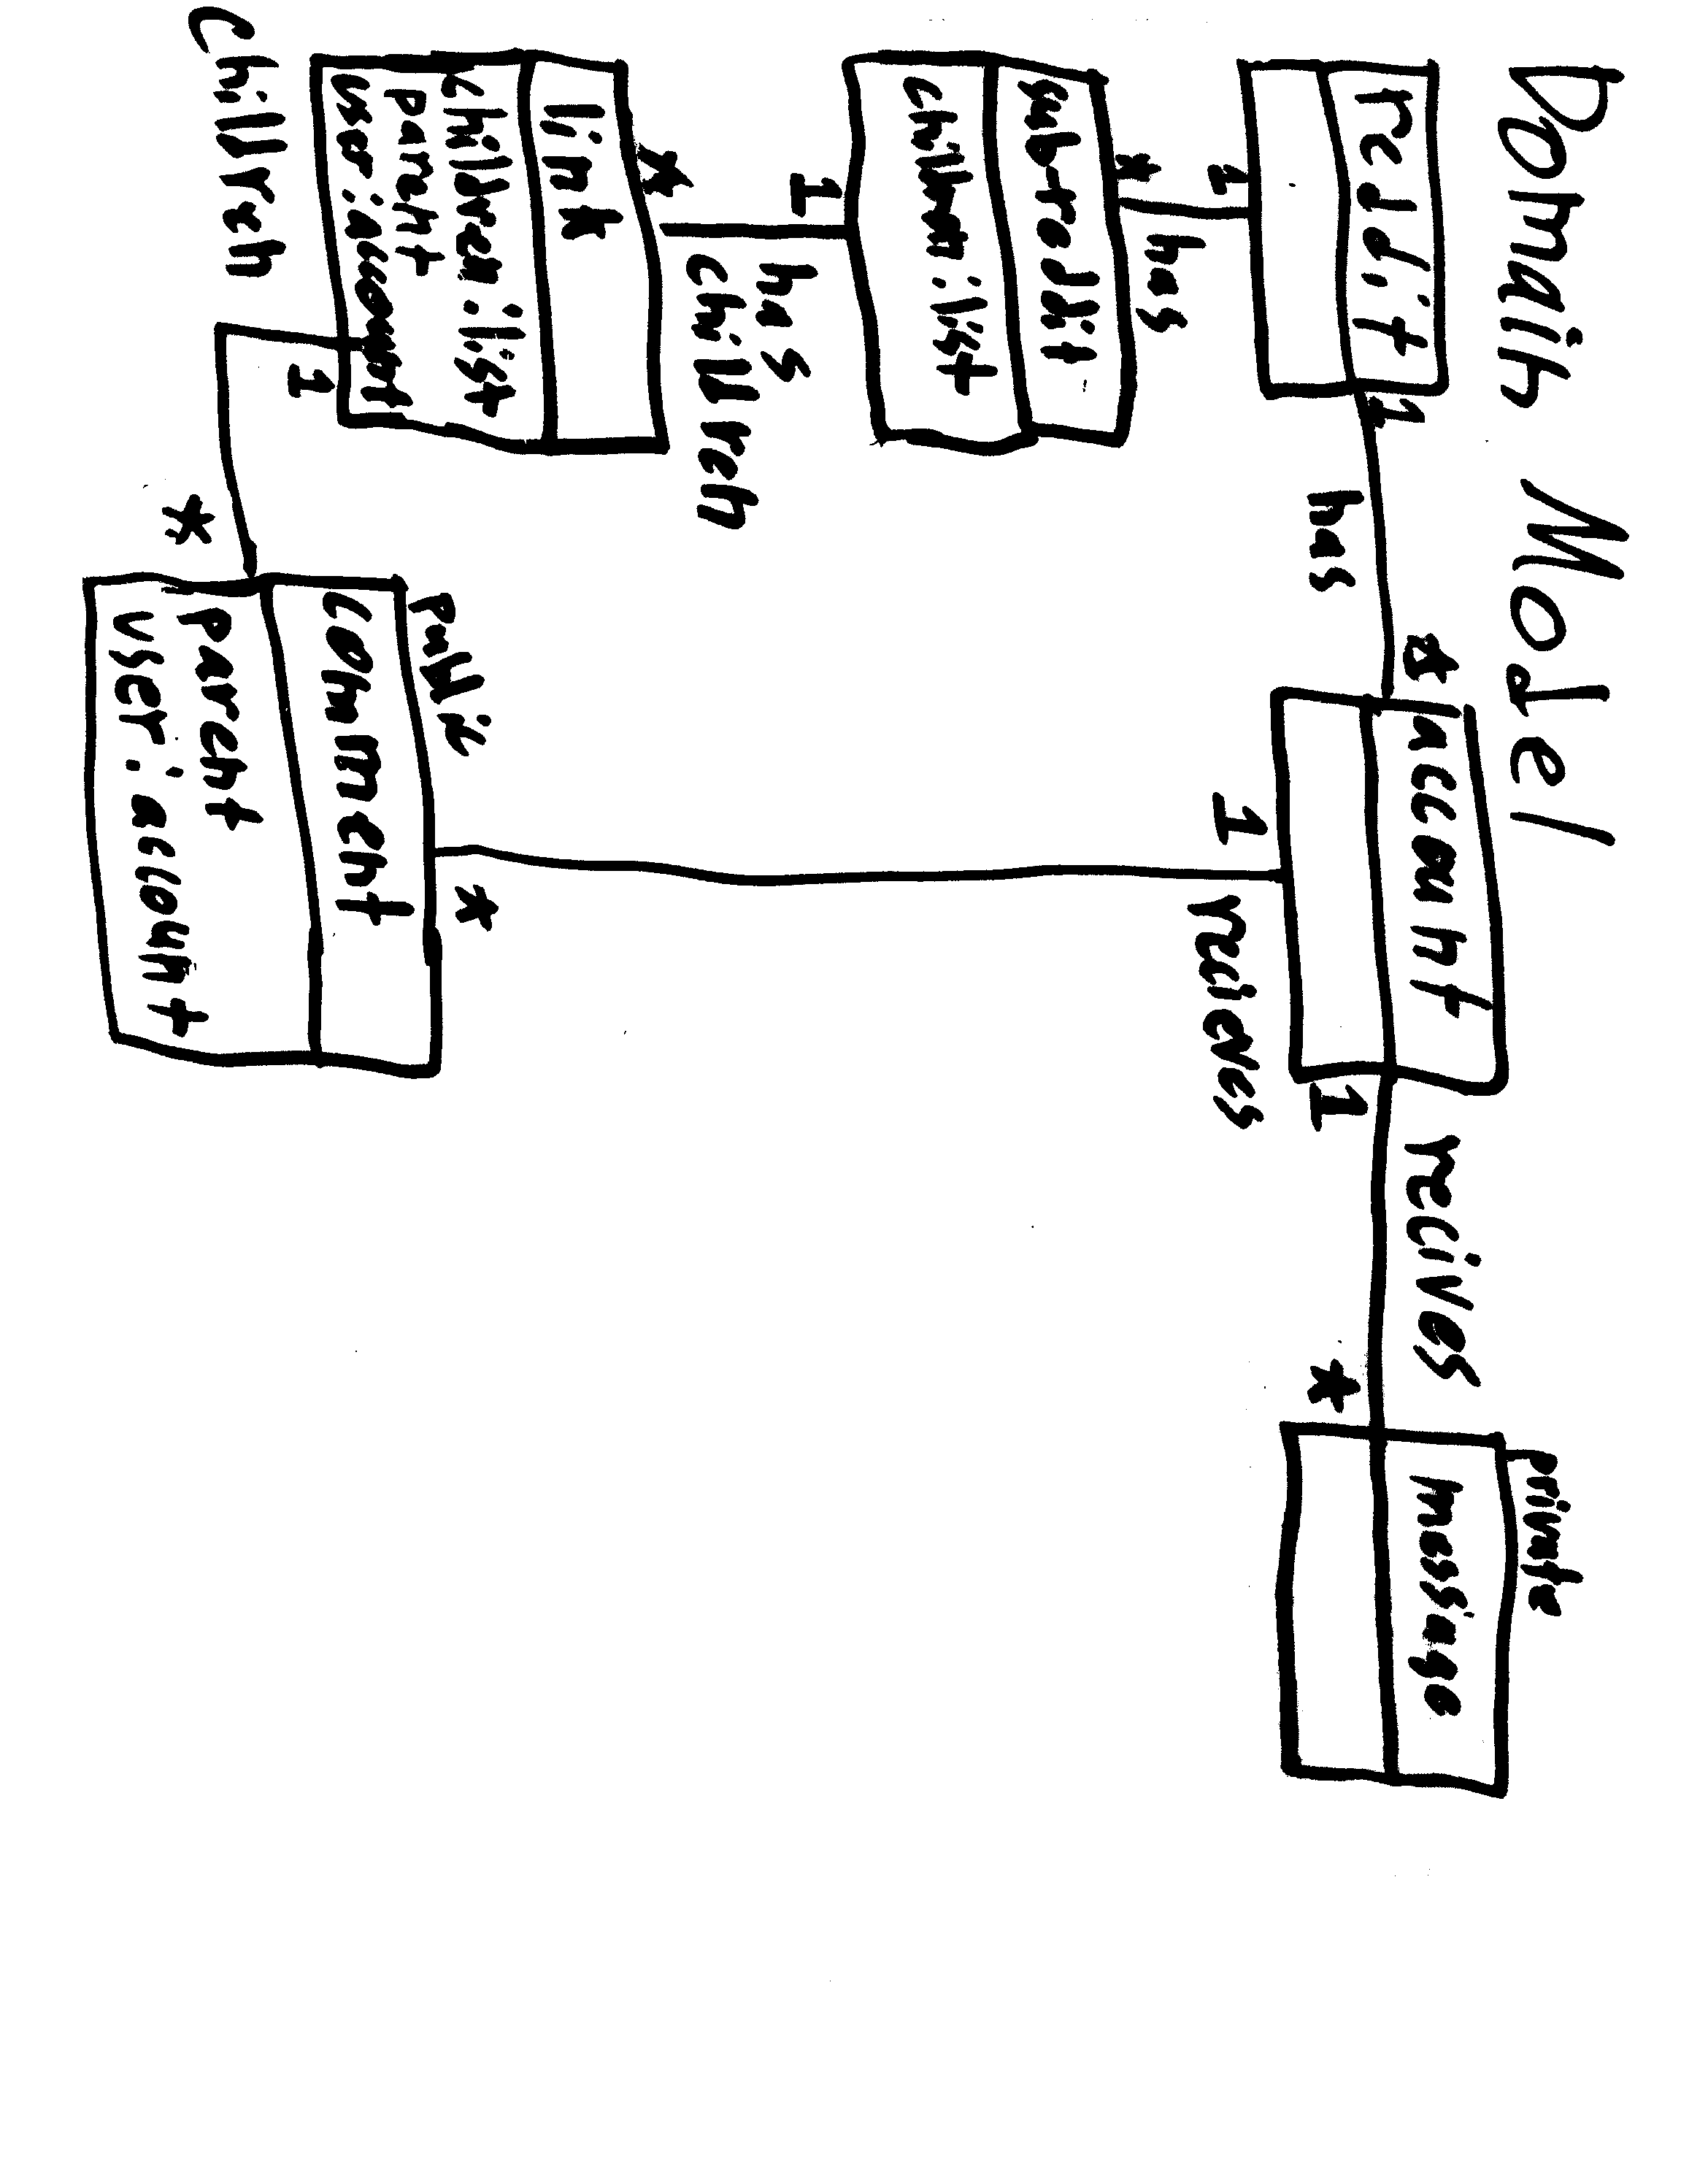
\includegraphics[width=0.8\textwidth]{domain.png}
\end{figure}

\clearpage
\section{Reading Data}
This sequence diagram would be very similar to all the other ones to get data from the website.
The difference would be what object we create in the middle, and what method we call to get information.
Notice how the session object must already be made to construct a different object.
\begin{figure}[ht]
	\centering
	\caption{Sequence Diagram Example for Getting Data}
	\label{sequence}
	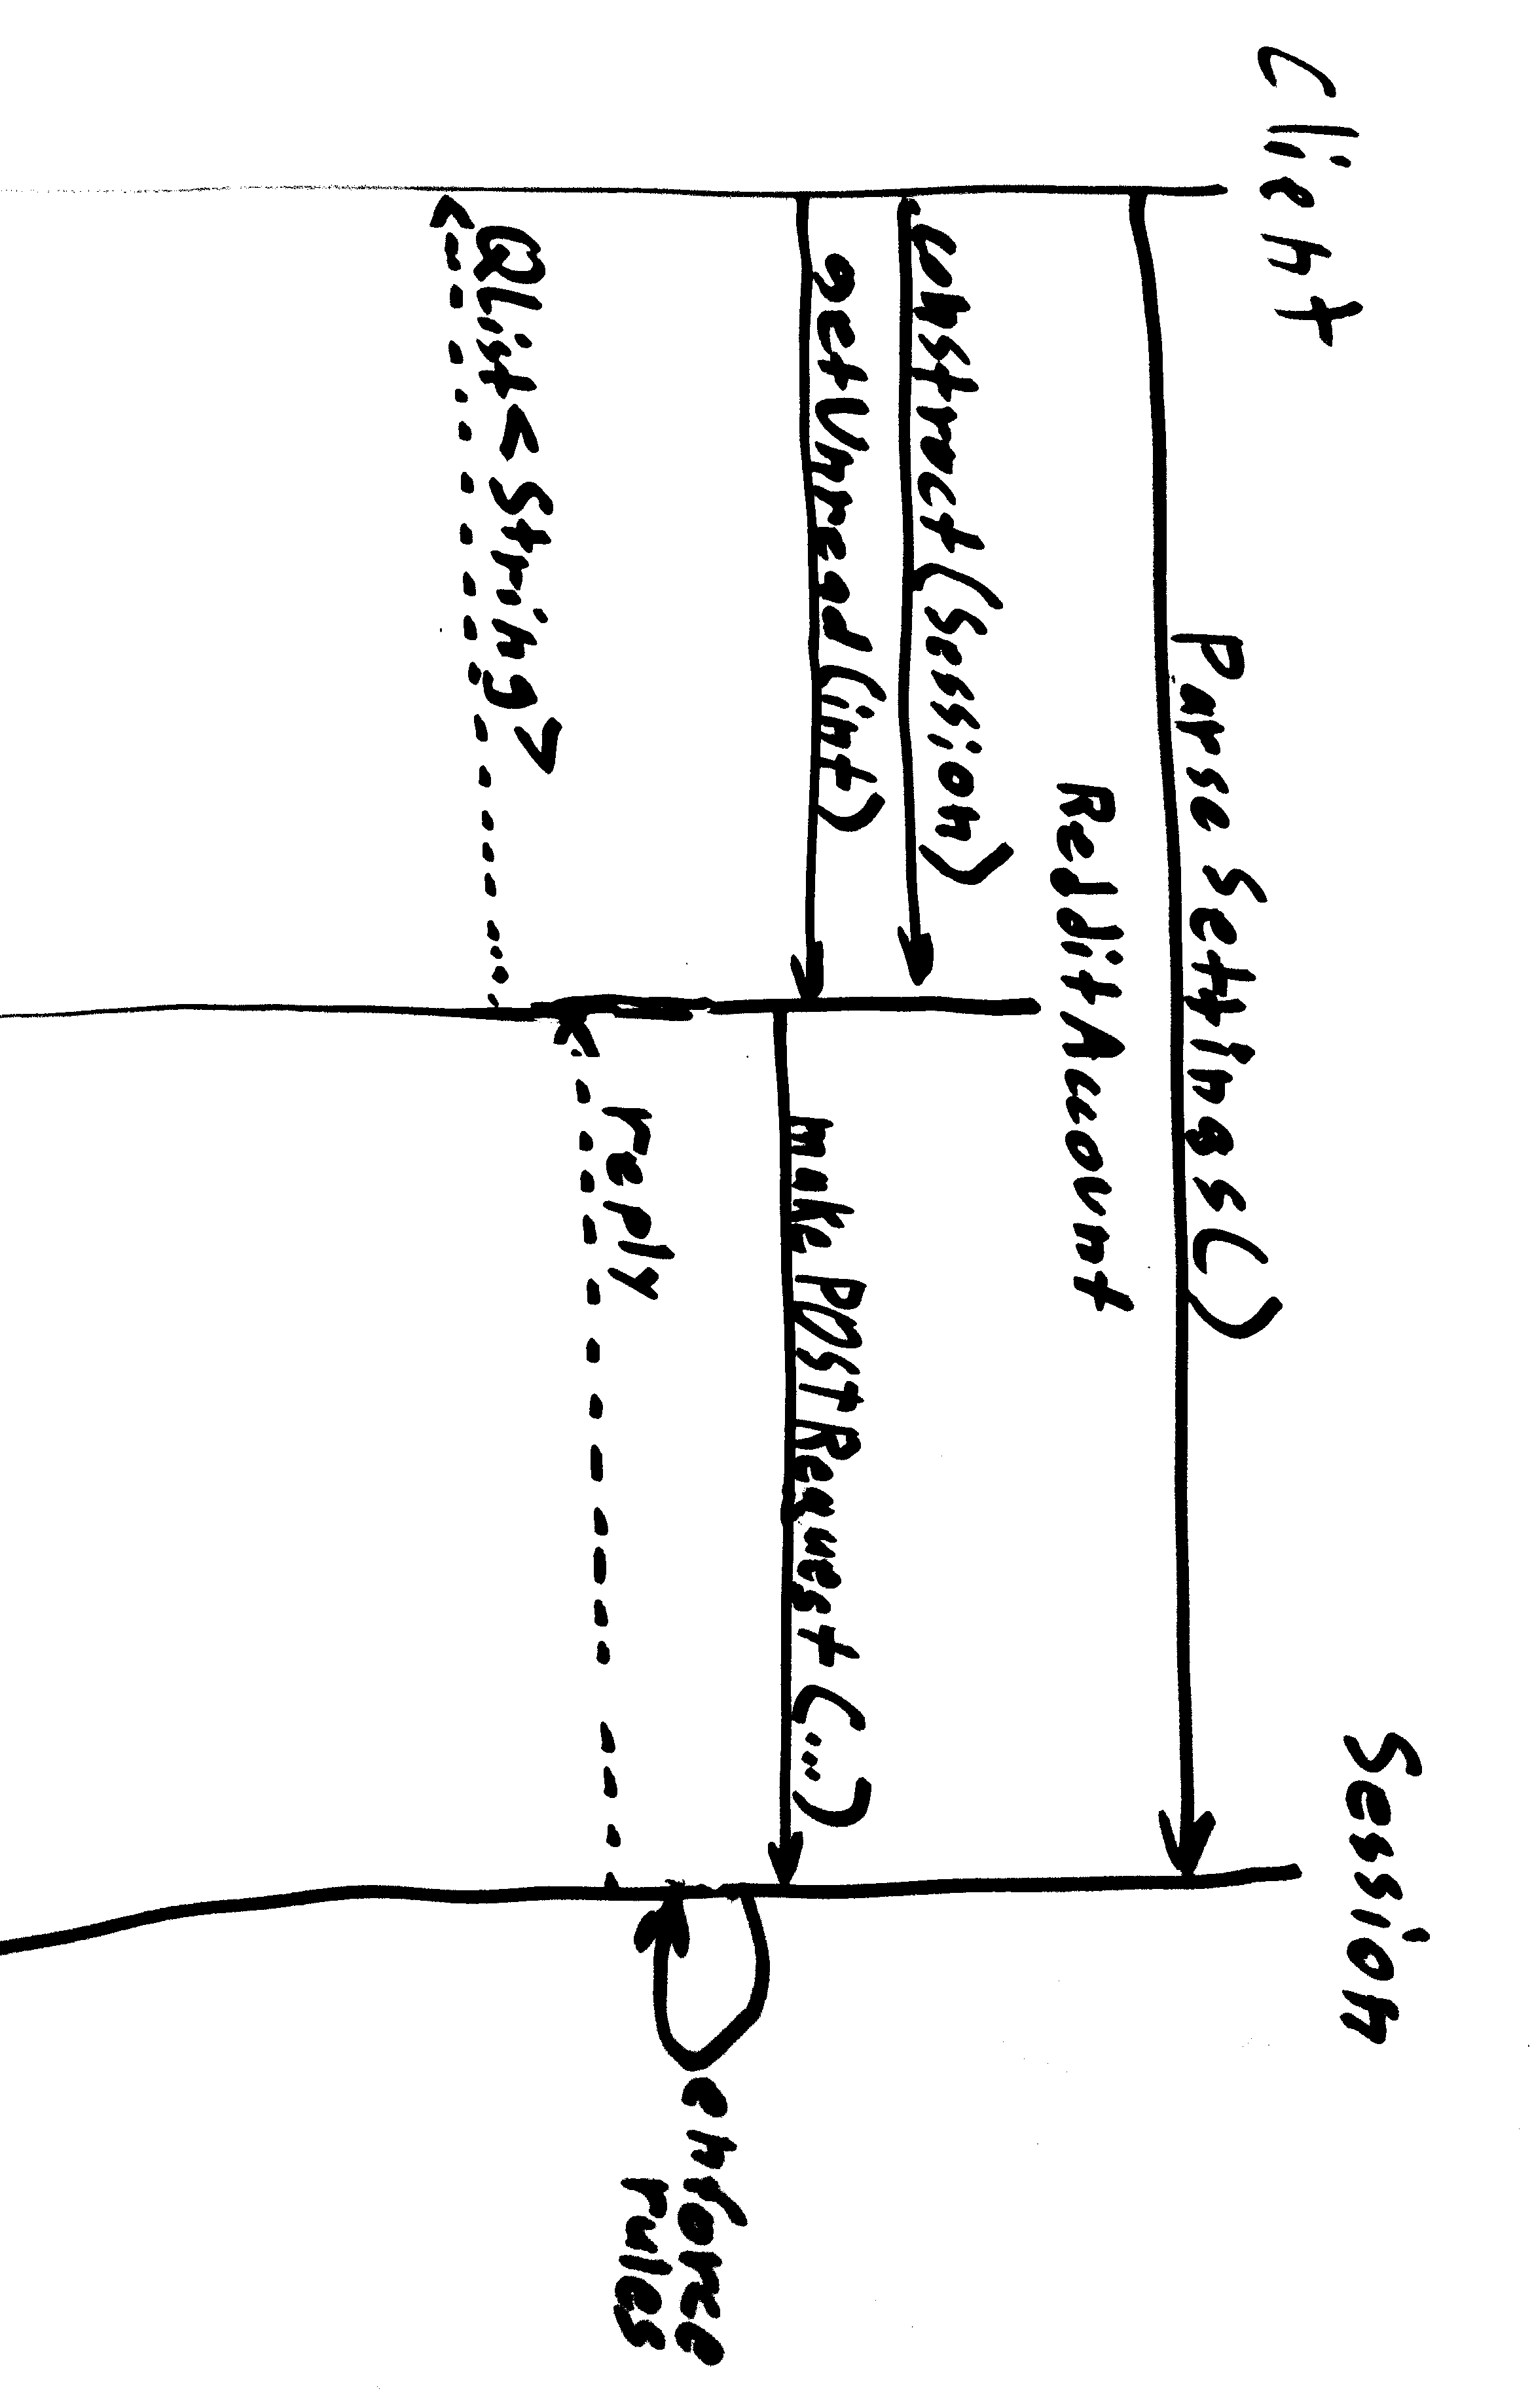
\includegraphics[width=0.65\textwidth]{sequence.png}
\end{figure}

\end{document}